\documentclass[aspectratio=1610]{beamer}

\setbeamertemplate{navigation symbols}{}

\usepackage[french]{babel}
\usepackage[utf8]{inputenc}
\usepackage[T1]{fontenc}
\usepackage{booktabs}
\usepackage{graphicx}
\usepackage{caption}
\usepackage{wrapfig}
\usepackage[export]{adjustbox}
\usepackage{hyperref}

\hypersetup{
    colorlinks=true,
    linkcolor=black,
    urlcolor=blue,
}

\usetheme{Madrid}

\graphicspath{ {./fractals/}{./mathematiciens/}{./cours/} }

\title[Les fractals]{Mandelbrot aux pays des fractals}

\author{Yann-Arby Bebba}
\institute[UPJV]{Université Picardie Jules Verne \\
\medskip
\textit{yann-arby.bebba@etud.u-picardie.fr}}
\date{\today}

\begin{document}

\begin{frame}
\titlepage    
\begin{figure}[h]
    \centering
    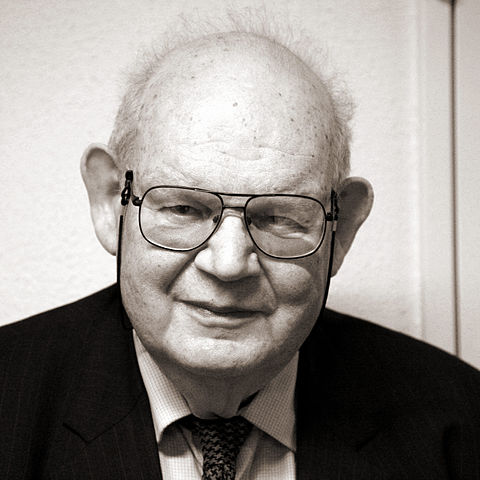
\includegraphics[width=3cm, height=3cm]{Benoit_Mandelbrot}
    {\caption*{Bênoit Mandelbrot en 2007}}
\end{figure}
\end{frame}

\begin{frame}
\frametitle{Table des matières}
\begin{minipage}{0.5\textwidth}
\tableofcontents
\end{minipage}%
\begin{minipage}{0.5\textwidth}
    \begin{figure}[h]
        \centering
        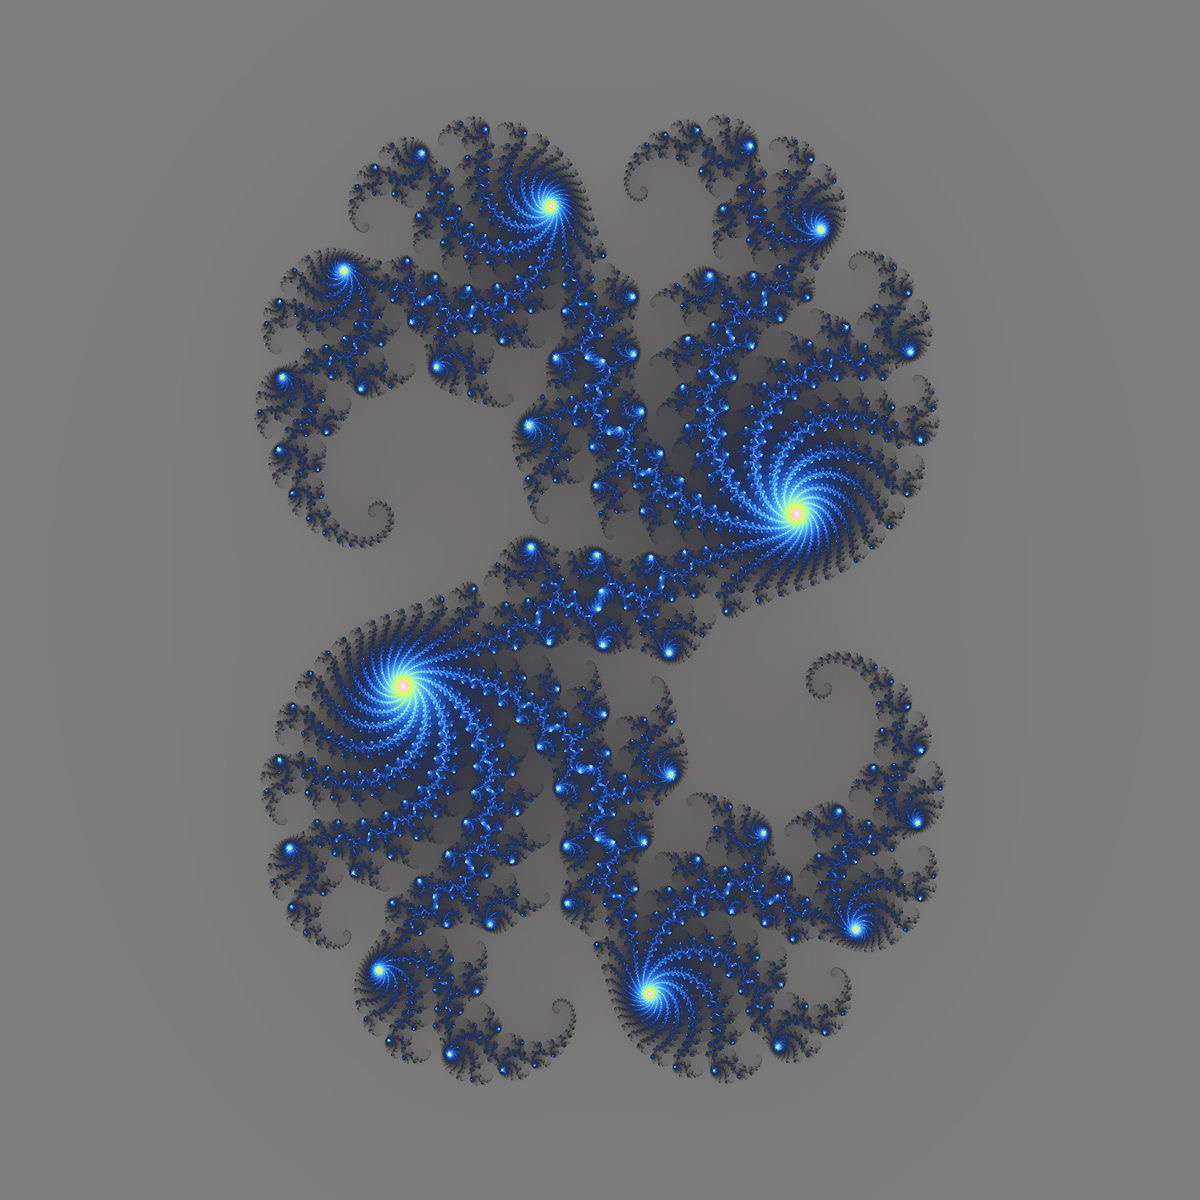
\includegraphics[width=1\textwidth]{fractal_4}
        {\caption*{Ensemble de Julia pour $c=0,285 + 0,013 i$.}}
        \label{fig: ensemble de Julia obtenu par itération inverse}
    \end{figure}
\end{minipage}
\end{frame}

\section{Chronologie}

\subsection{Les pères fondateurs}

\begin{frame}
\frametitle{Les pères fondateurs}
\begin{minipage}[t]{0.8\textwidth}
    \begin{flushleft}
\begin{itemize}
    \item Euclide d'Alexandrie (vers 300 avant J.-C.) :
 
        il définit la géométrie qui va prévaloir durant les deux millénaires à venir.
    \item Gaston Julia (1893-1929) étudiant de Poincaré et 

Pierre Fatou (1878-1929) :

        Vers 1914, les deux mathématiciens s'intéressent aux images répétées (itérations).Travaux méconnus car les résultats ne sont apparents que par le grand nombre de points et le grand nombre d'itérations, impossible à révéler sans l'aide d'ordinateurs. Gaston Julia publie ses travaux en 1918, il y met en évidence ce qui est connu aujourd'hui sous le nom d'ensemble de Julia: des bassins d'attraction aux frontières très tourmentées. Il les imagine mais ne les verra jamais faute de disposer de moyens de calcul comme les ordinateurs. Ses travaux attendront cinquante ans avant d'être exploités.

\end{itemize}
    \end{flushleft}
\end{minipage}%
\begin{minipage}[t]{0.2\textwidth}
    \begin{figure}[h]
        \centering
        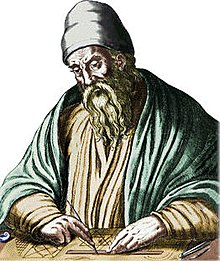
\includegraphics[width=0.7\textwidth]{Euclide-Alexandrie}
    {\caption*{Euclide Alexandrie}}
        \label{fig: Euclide Alexandrie}
    \end{figure}
     \begin{figure}[h]
        \centering
        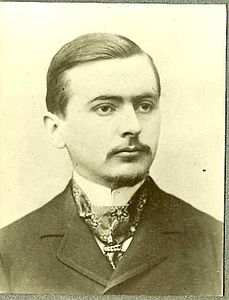
\includegraphics[width=0.8\textwidth]{Pierre_Fatou}
     {\caption*{Pierre Fatou}}
        \label{fig:Pierre Fatou}
     \end{figure}
    \end{minipage}

\end{frame}

    \begin{frame}
        \begin{minipage}{0.8\textwidth}
            \begin{itemize}
    \item Benoît Mandelbrot (1924-2010) Mathématicien polonais franco-américain:

        En 1975, il invente le fractal. Il est considéré comme le père de la géométrie fractale.

        A l'époque il travaille chez IBM et résout un problème de bruit aléatoire dans les transmissions entre ordinateurs.
        Il avait constaté que les erreurs étaient de type fractal.

 Il prend connaissance des oeuvres de Julia et Fatou et les exploite à l'aide d'ordinateurs. Il s'intéresse à une itération particulièrement simple : en partant d'un point complexe du plan, un nouveau point pour $z$ du plan est calculé en prenant le carré du précédent ajouté d'une constante. Ainsi naquît la célèbre formule $z\to z^2+c$, qui donna naissance au monde merveilleux des fractales.
            \end{itemize}
        \end{minipage}%
        \begin{minipage}{0.2\textwidth}
         \begin{figure}[h]
        \centering
        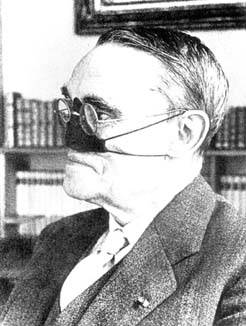
\includegraphics[width=0.7\textwidth]{gaston-julia}
        {\caption*{Gaston Julia}}
        \label{fig:Gason Julia}
    \end{figure}
           
        \end{minipage}
    \end{frame}


\section{Définition d'un fractal}

\begin{frame}
\frametitle{Définition d'un fractal}
Comme point de départ, nous prendrons la définition suivante d'un fractal.
\begin{block}{Définition}
Un fractal est un objet qui a les trois propriétés suivantes:
\begin{itemize}
    \item irrégulier à toutes les échelles;
    \item auto-similaire;
    \item de dimension non-entière.
\end{itemize}
\end{block}
\begin{minipage}{0.3\textwidth}
\begin{figure}[h]
    \centering
    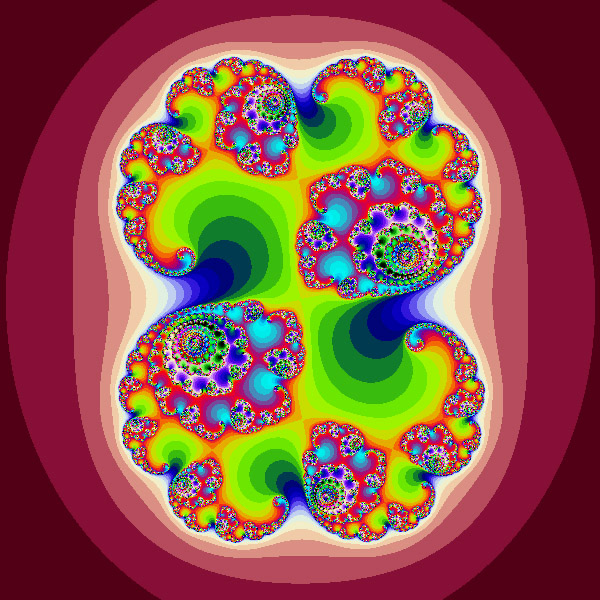
\includegraphics[width=4cm, height=4cm]{fractal_7}
    \label{fig:fractal_7}
\end{figure}
\end{minipage}%
\begin{minipage}{0.4\textwidth}
    \begin{figure}[h]
        \centering
        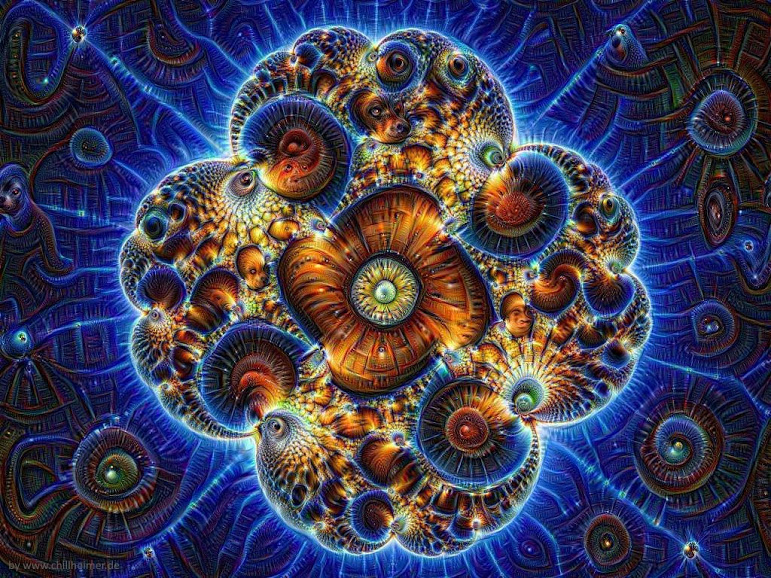
\includegraphics[width=5cm, height=4cm]{fractal-wallpaper}
        \label{fig:fractal-wallpaper}
    \end{figure} 
\end{minipage}%
\begin{minipage}{0.3\textwidth}
    \begin{figure}[h]
        \centering
        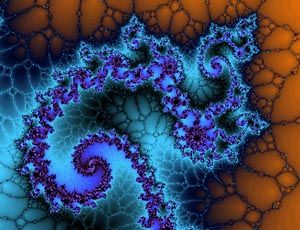
\includegraphics[width=4cm, height=4cm]{zbulle3}
        \label{fig:mfractal}
    \end{figure} 
\end{minipage}
\end{frame}

\subsection{Irrégulier à toutes les échelles}
\begin{frame}
\frametitle{Irrégulier à toutes les échelles}

\begin{minipage}{0.6\textwidth}
\begin{block}{Définition}
    Un objet est irrégulier à toutes les échelles si, même en le regardant de plus en plus près, il apparaît toujours irrégulier.
\end{block}
\begin{figure}[h]
    \centering
    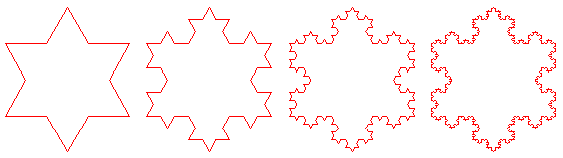
\includegraphics[width=0.8\textwidth]{flocon}
    {\caption*{Exemple du flocon de neige de von Koch}}
    \label{fig:flocon}
\end{figure}
\end{minipage}%
\begin{minipage}{0.4\textwidth}
    \begin{figure}[h]
        \centering
        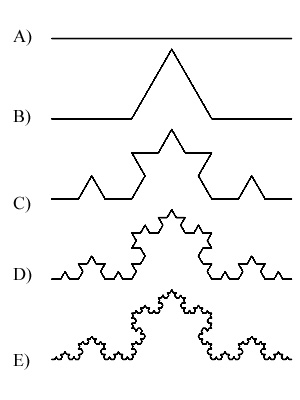
\includegraphics[width=0.8\textwidth]{courbe_de_von_koch}
        {\caption*{Exemple de la courbe de von Koch}}
        \label{fig:courbe_de_von_koch}
    \end{figure}
\end{minipage}
\end{frame}
\subsection{Auto-similitude}
\begin{frame}
\frametitle{Auto-similitude}
\begin{block}{Définition}
    Un objet $F$ est auto-similaire s'il se décompose en un nombre fini de parties $F_1, \ldots , F_{N}$ qui sont toutes similaires à l'objet entier $F$. Une partie $F_{i}$ est similaire à $F$ s'il existe un facteur de dilatation s tel que si l'on dilate $F_{i}$ d'un facteur $s$, on retrouve $F$ au complet.
\end{block} 
\begin{description}
\begin{minipage}{0.5\textwidth}
    \item[a)] \textbf{Segment} 
      \begin{figure}[h]
          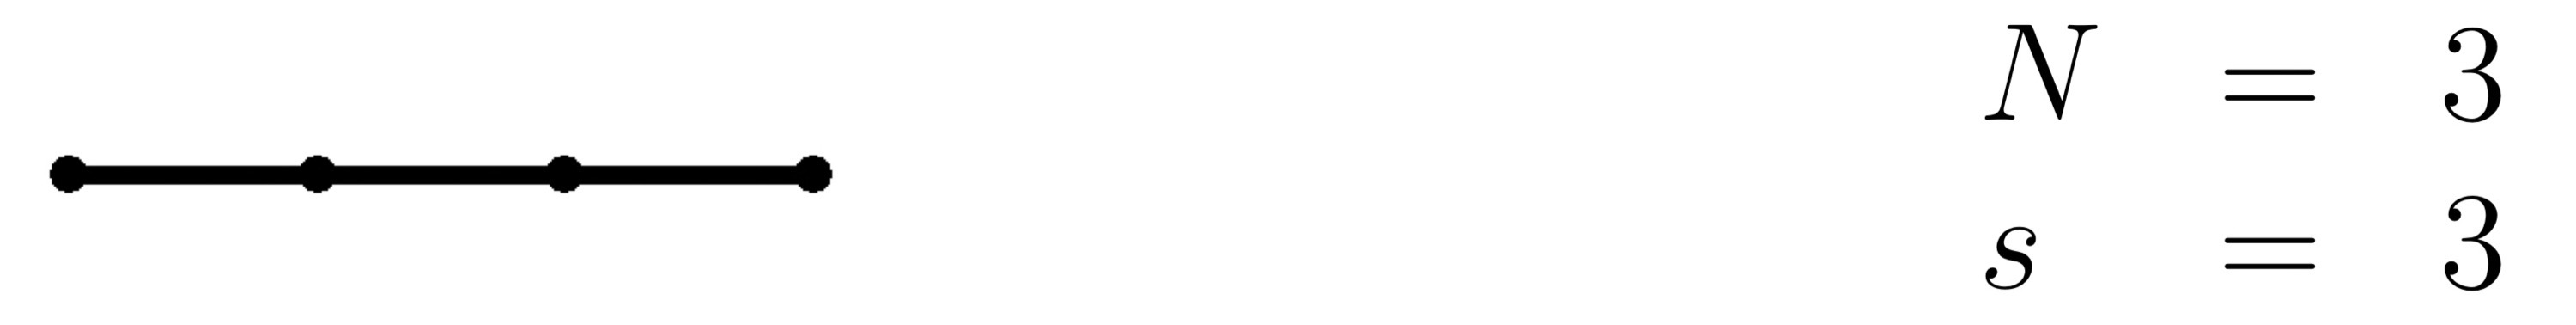
\includegraphics[width=0.6\textwidth,left]{IMG_1483}
          \label{fig:public1}
      \end{figure} 
 
    \item[b)] \textbf{Carré} 
    \begin{figure}[h]
        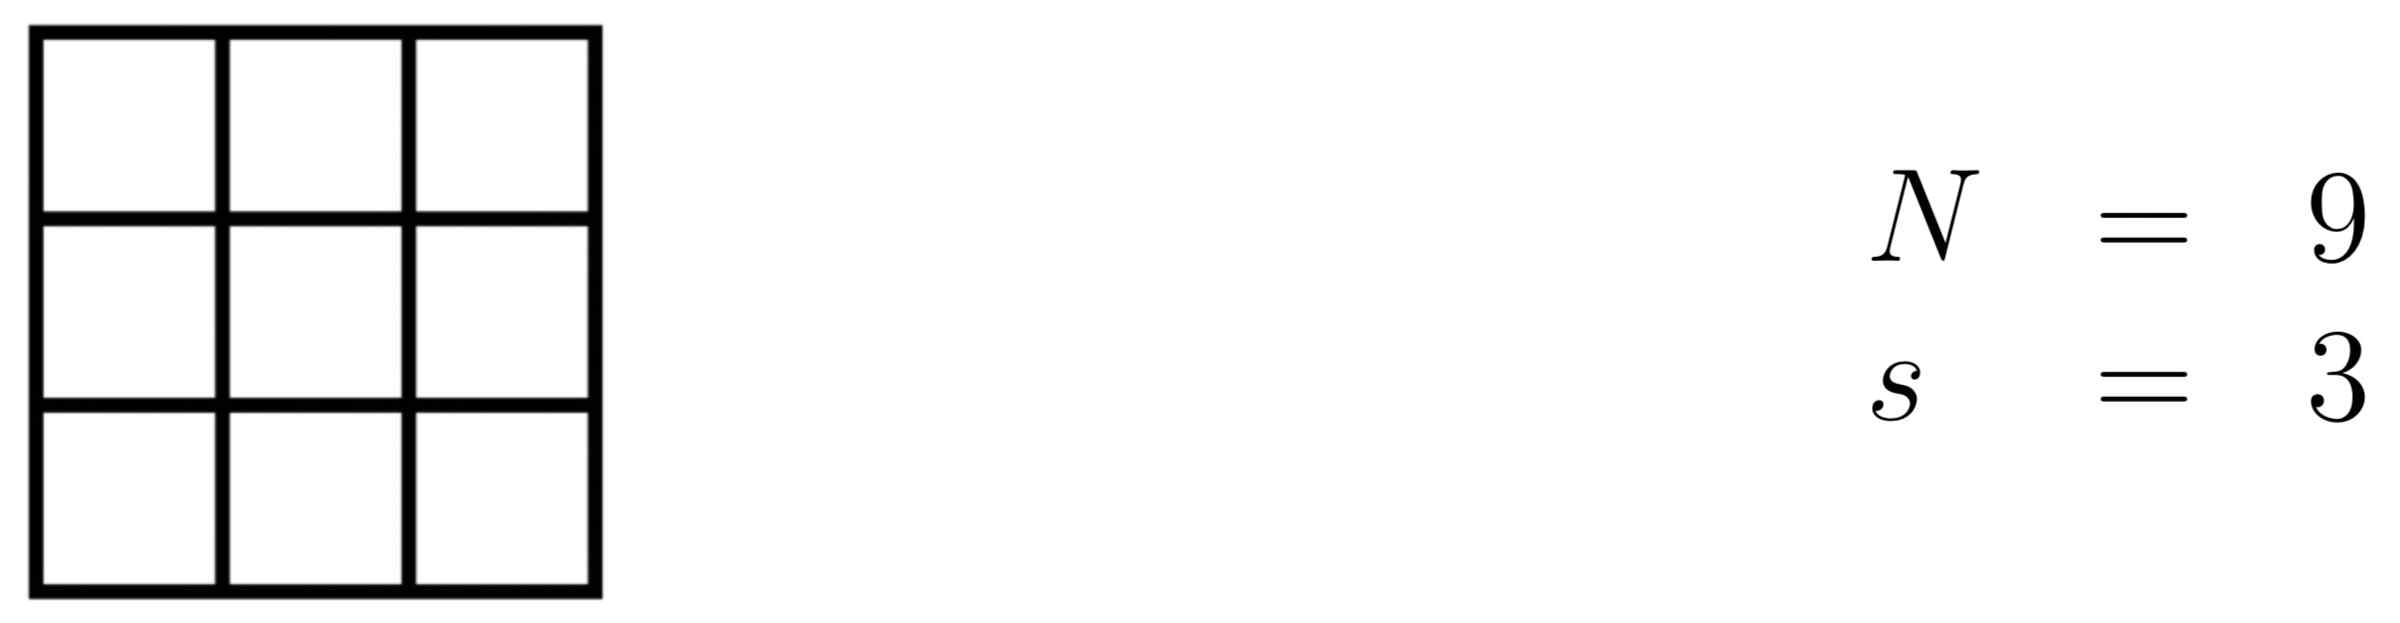
\includegraphics[width=0.6\textwidth,left]{IMG_1484}
        \label{fig:IMG_1484}
    \end{figure}    

\end{minipage}%
\begin{minipage}{0.5\textwidth}
    \item[c)] \textbf{Cube} 
    \begin{figure}[h]
        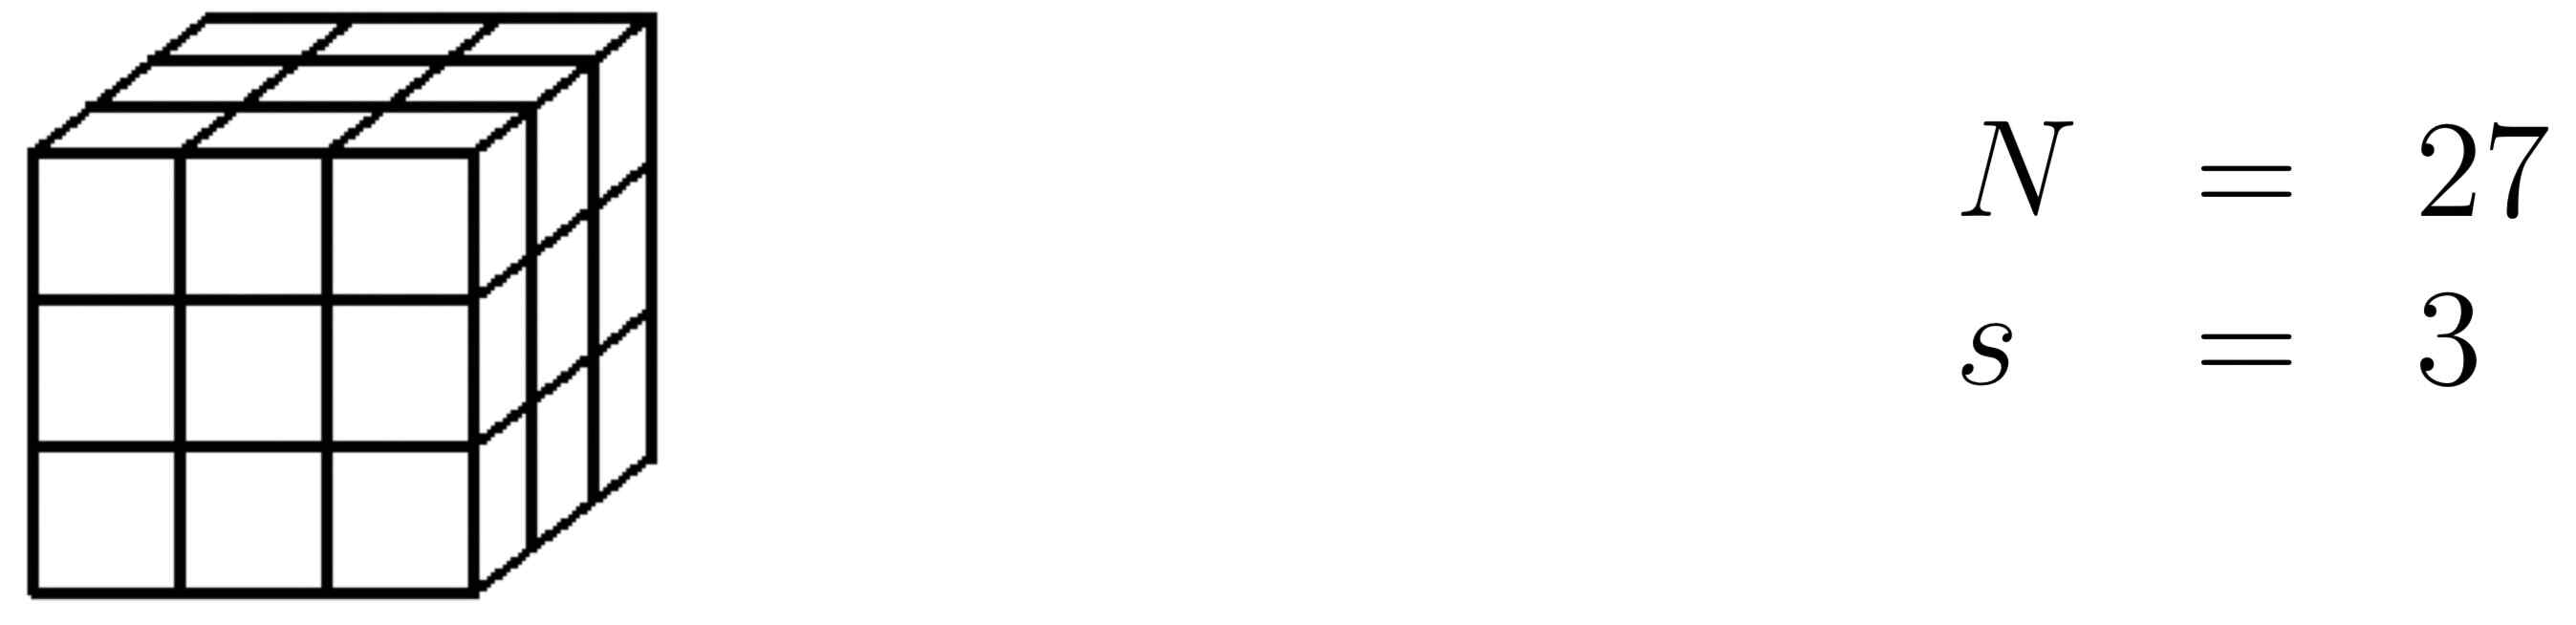
\includegraphics[width=0.6\textwidth,left]{IMG_1485}
        \label{fig:IMG_1483}
    \end{figure}    

    \item[d)] \textbf{Courbe de von Koch}
    \begin{figure}[h]
        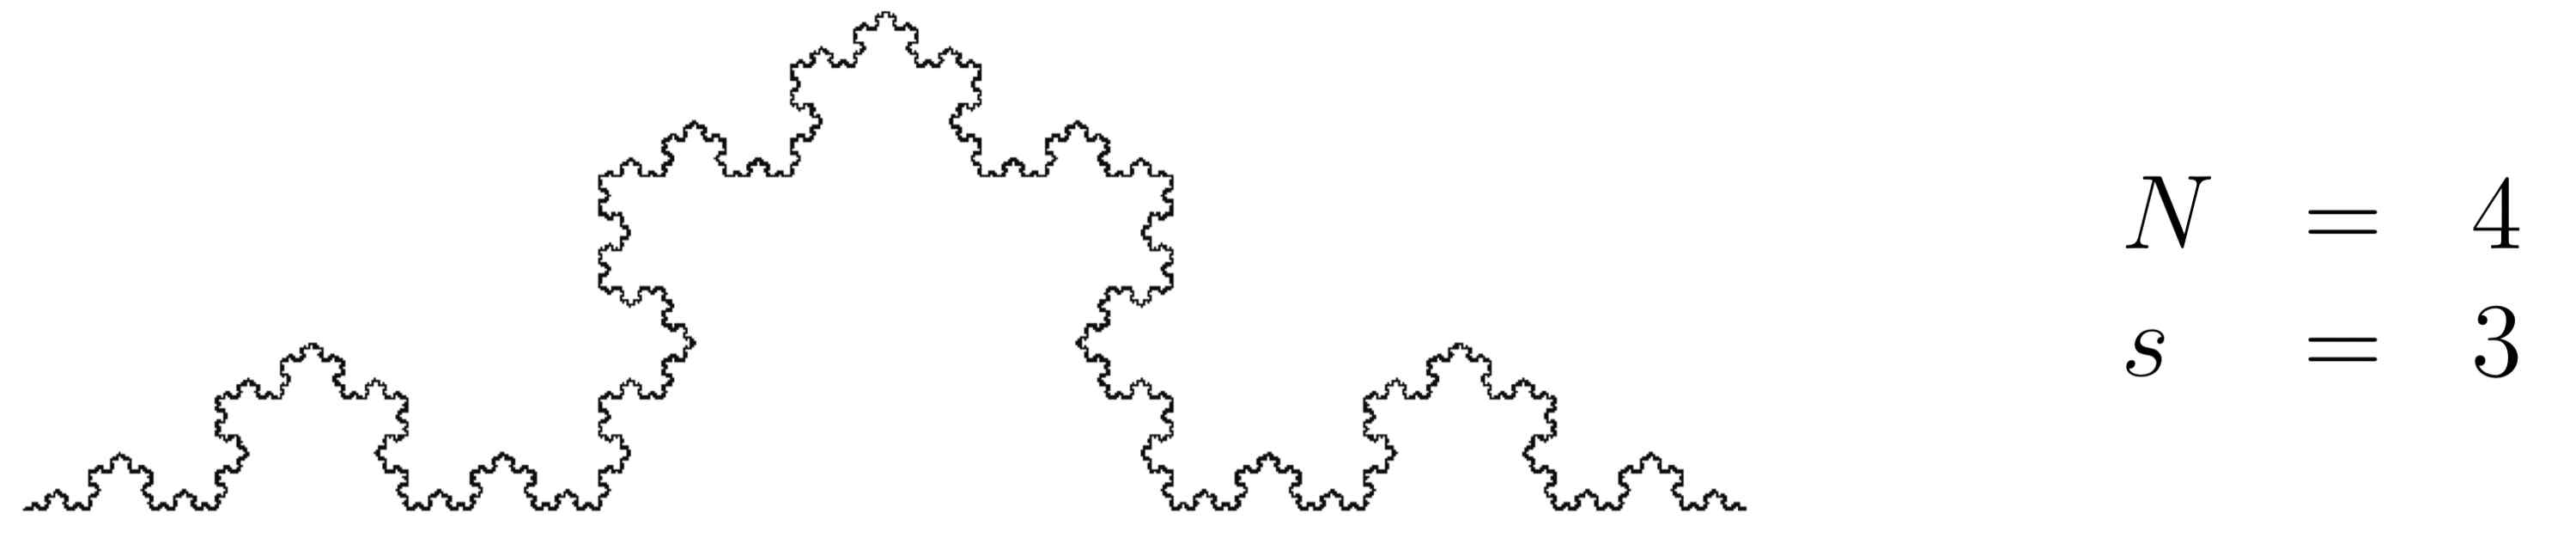
\includegraphics[width=0.7\textwidth,left]{IMG_1486}
        \label{fig:IMG_1486}
    \end{figure} 

\end{minipage}
\end{description} 
\end{frame}

\begin{frame}
\begin{description}
    \item[e)] \textbf{Triangle de Sierpinski}
\begin{minipage}[b]{0.4\textwidth}
 Voici les premières étapes de

 construction 
\begin{figure}[h]
        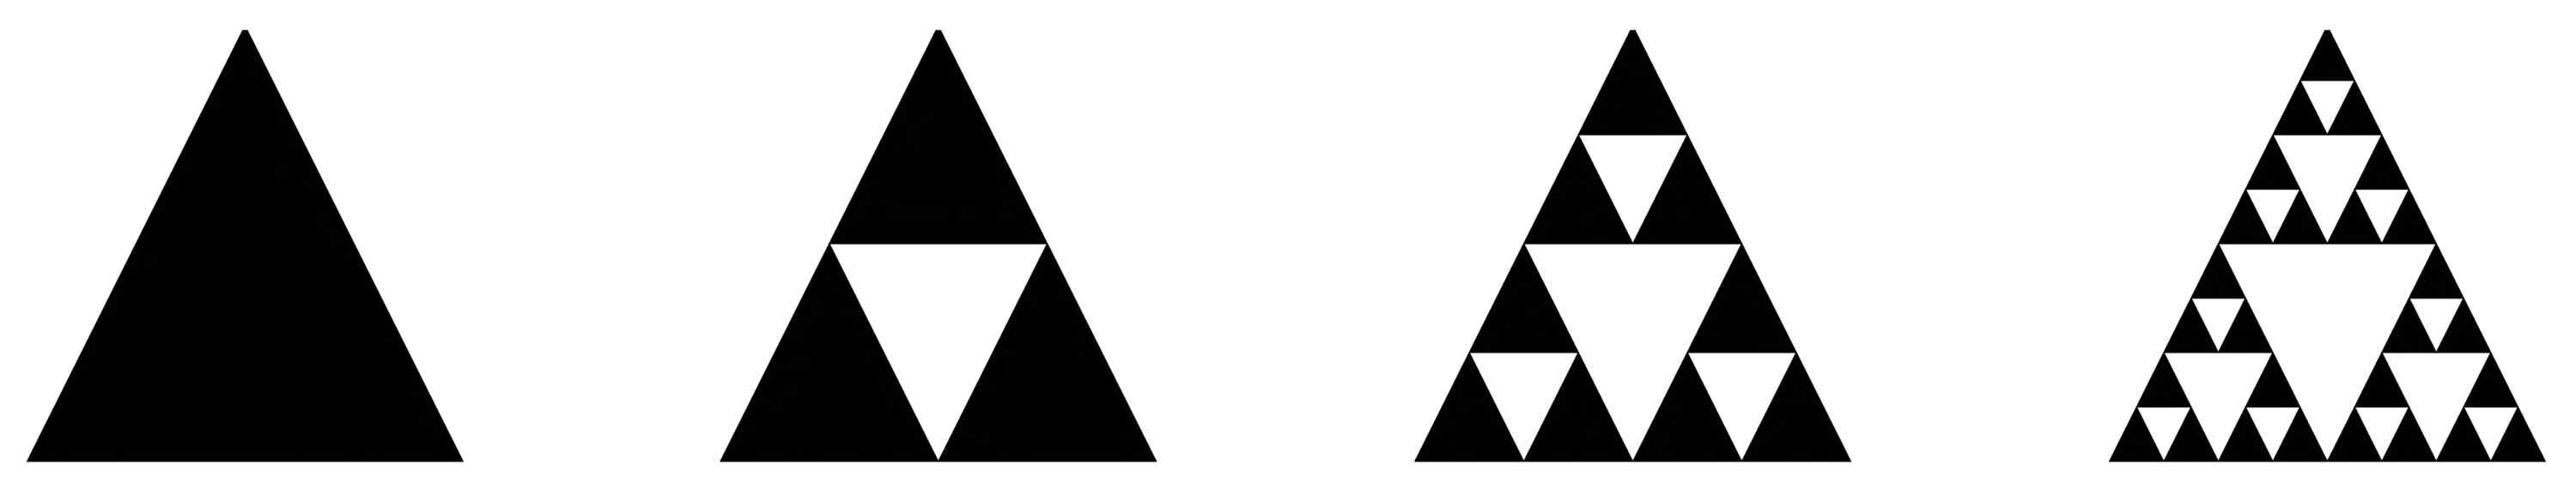
\includegraphics[width=0.8\textwidth,left]{IMG_1487}
        \label{fig:IMG_1487}
    \end{figure}
\end{minipage}%
\begin{minipage}[b]{0.5\textwidth}
en itérant à l'infini ce processus
\begin{figure}[h]
        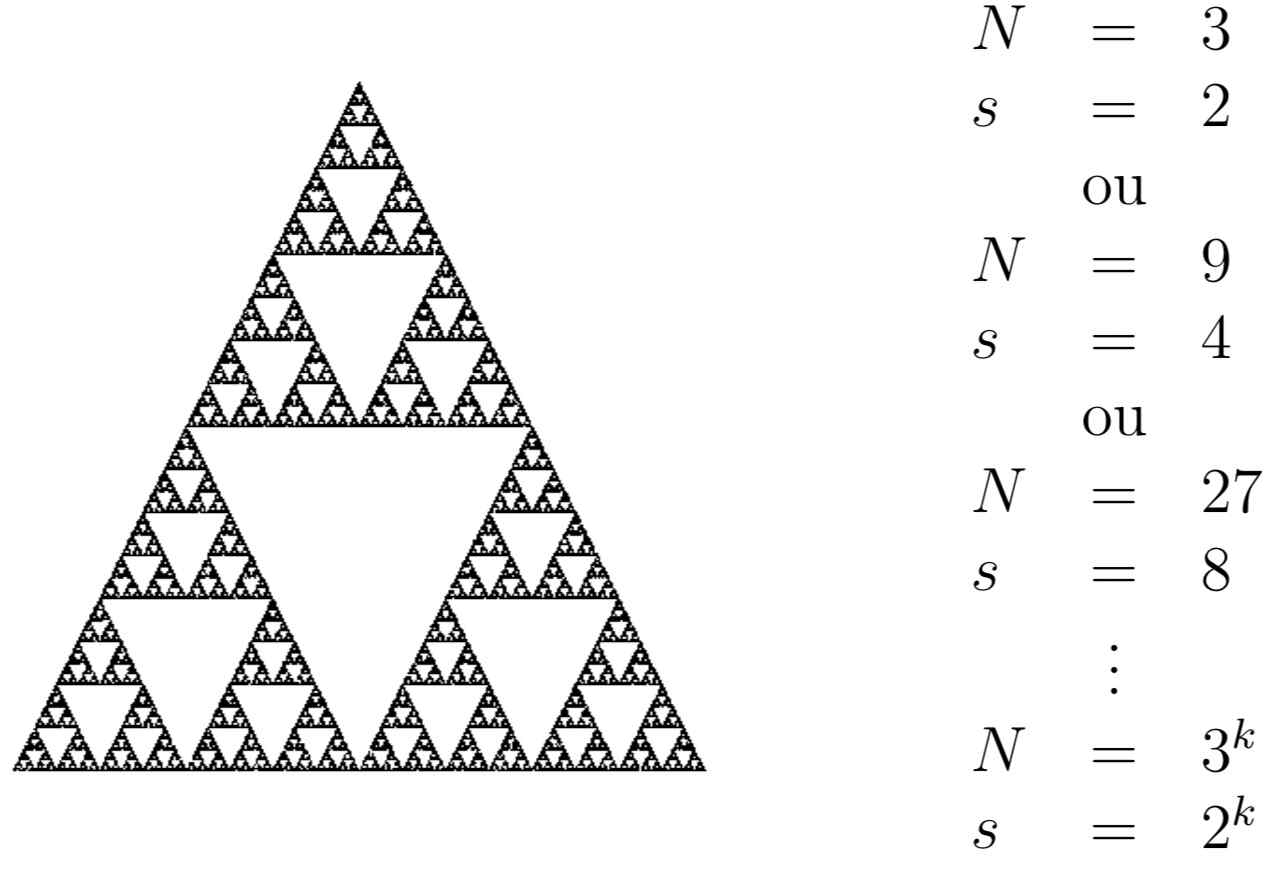
\includegraphics[width=5cm,height=3cm,left]{IMG_1488}
        \label{fig:IMG_1488}
    \end{figure}
\end{minipage}
\end{description}
\textbf{On peut préciser et généraliser la définition d'auto-similitude}
 \begin{block}{Définition}
    Une similitude du plan est une application $ w: \mathbb{R}^{2} \to \mathbb{R}^{2} $ telle que $\|w(P)-w(Q)\|=k\|P-Q\|$ pour tout $P \in \mathbb{R}^{2}$ et pour tout $Q\in \mathbb{R}^{2}$ où $k$ est une constante appelée le rapport de la similitude $w$.
\end{block}
\begin{block}{Définition}
    Un ensemble $F\subset \mathbb{R}^{2}$ est auto-similaire s'il existe des similitudes $w_1, \ldots , w_{N}$ telles que $F=w_1(F)\cup \ldots \cup w_{N}(F)$
\end{block}
\end{frame}

\subsection{Dimension de similitude}
\begin{frame}
\frametitle{Dimension de similitude}
\begin{description}
\begin{minipage}[b]{0.3\textwidth}
    \item[] \textbf{Dimension 1}
    \begin{figure}[h]
        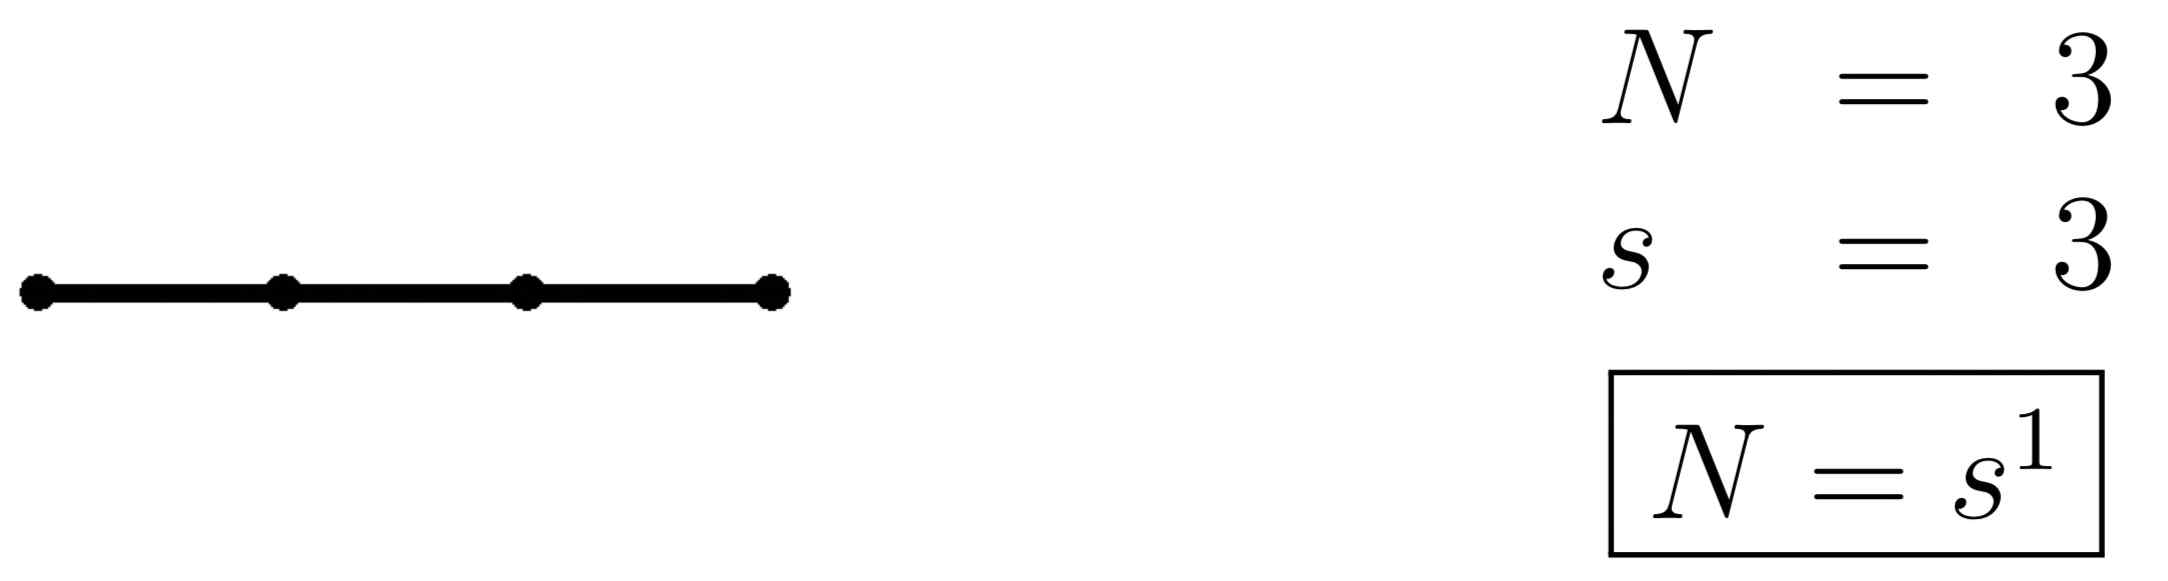
\includegraphics[width=0.7\textwidth,left]{IMG_1489}
        \label{fig:IMG_1489}
    \end{figure}
\end{minipage}%
\begin{minipage}[b]{0.3\textwidth}
    \item[] \textbf{Dimension 2}
    \begin{figure}[h]
        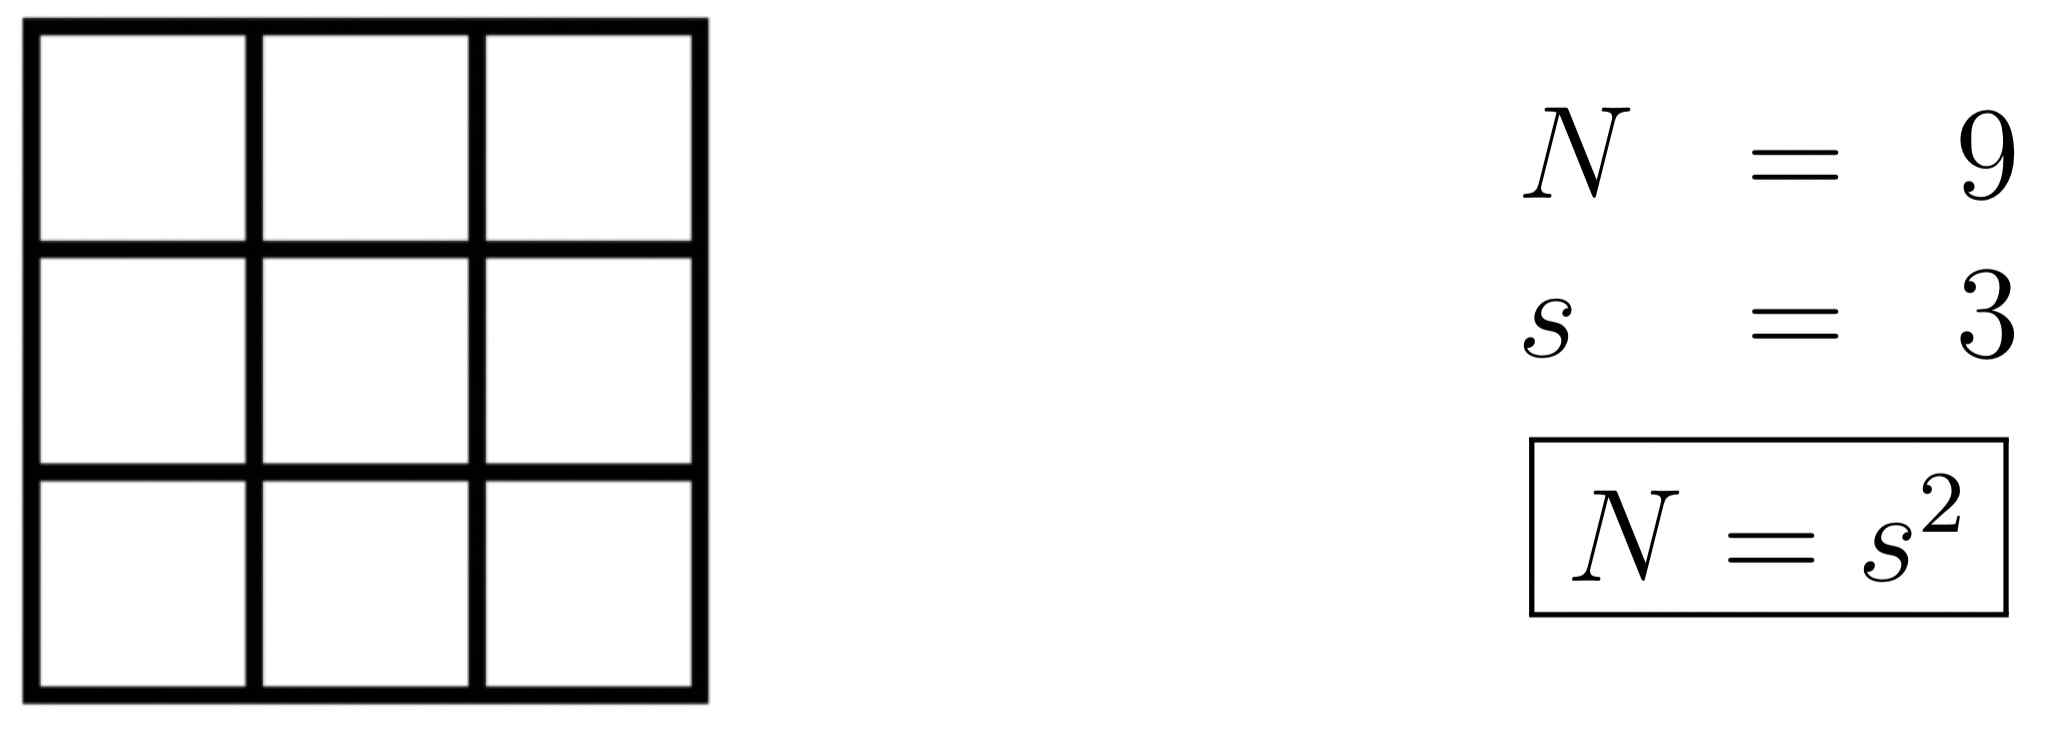
\includegraphics[width=0.7\textwidth,left]{IMG_1490}
        \label{fig:IMG_1490}
    \end{figure}
\end{minipage}%
\begin{minipage}[b]{0.3\textwidth}
    \item[] \textbf{Dimension 3}
    \begin{figure}[h]
        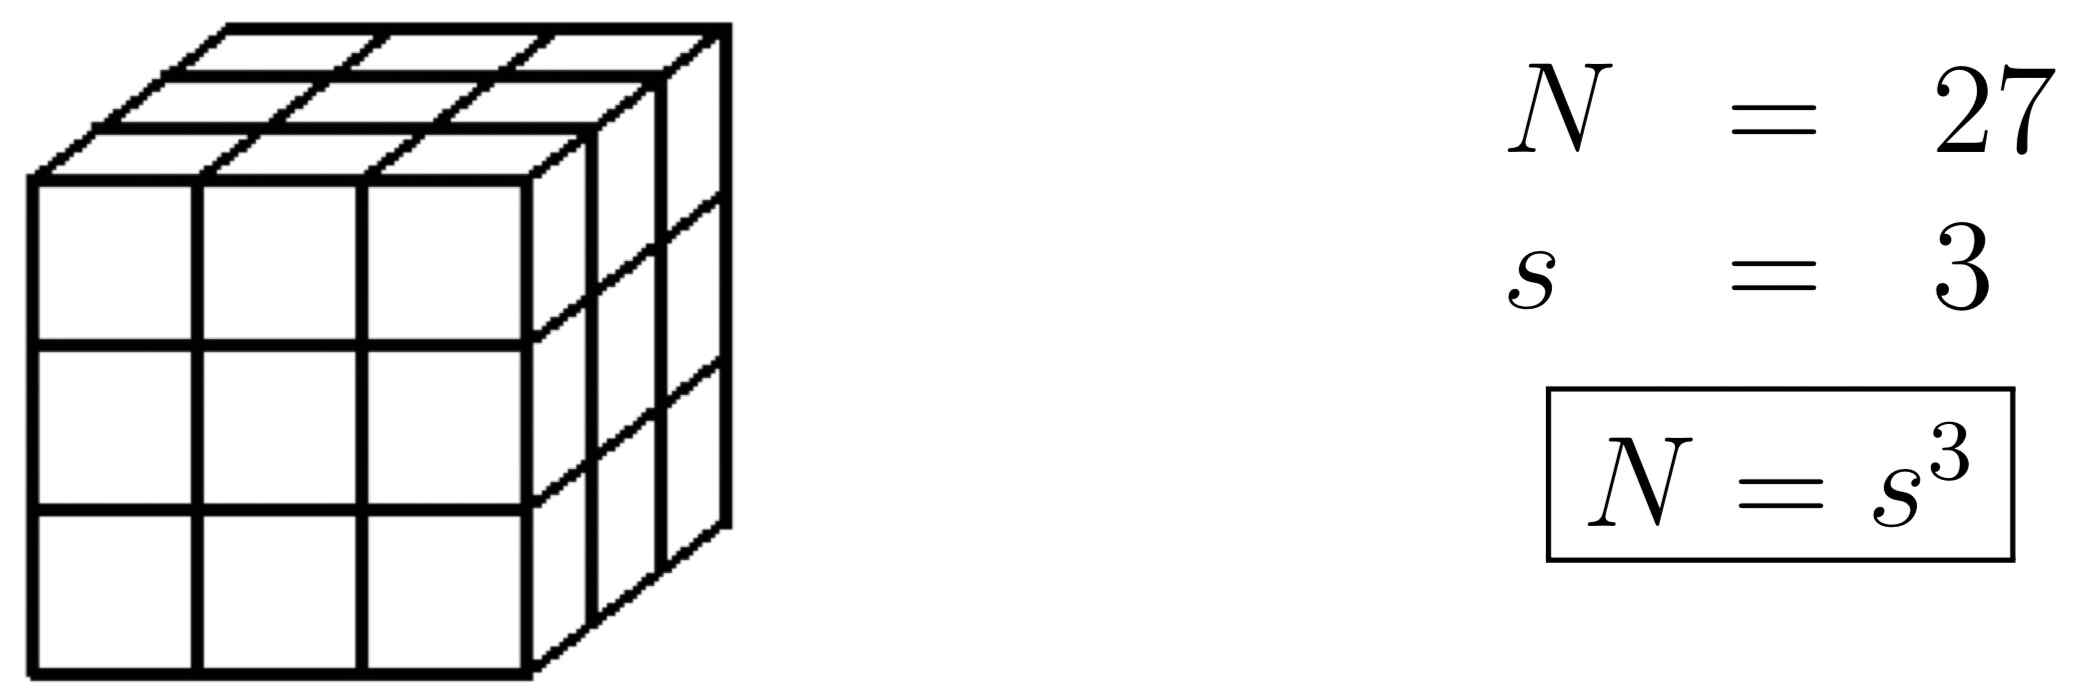
\includegraphics[width=0.7\textwidth,left]{IMG_1491}
        \label{fig:IMG_1491}
    \end{figure}
\end{minipage}
\end{description}
Peu importe le facteur de dilatation $s$, on aura toujours  $N=s^{d}$, où $d$ est la dimension.
\begin{block}{Définition}
    La dimension de similitude d'un objet auto-similaire se décomposant en $N$ parties similaires à l'objet par un facteur de dilatation s est $d=\frac{\log N}{\log s}$.
\end{block}    
\textbf{Dimension de la courbe de von Koch} :

\begin{minipage}{0.5\textwidth}
\begin{figure}[h]
    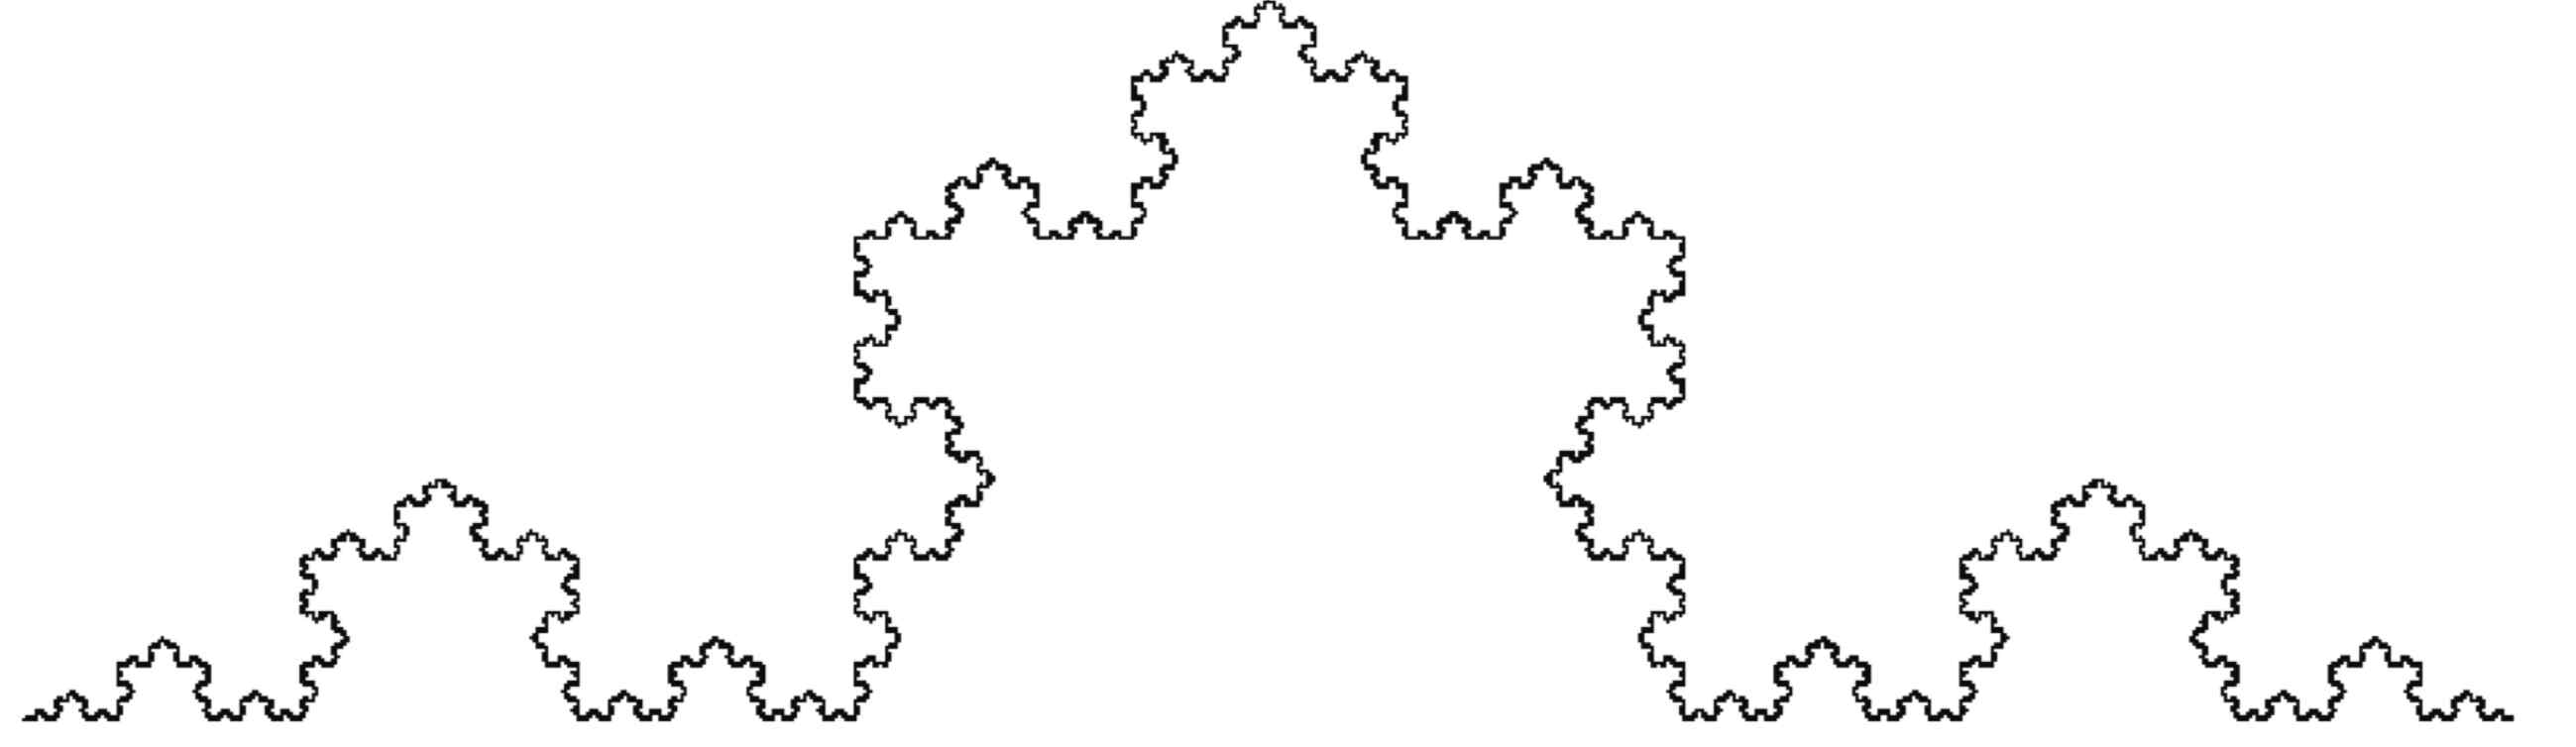
\includegraphics[width=0.7\textwidth,left]{IMG_1492}
    \label{fig:IMG_1492}
\end{figure}
\end{minipage}%
\begin{minipage}{0.5\textwidth}
\raggedright
On a $N=4$ et $s=3$. Ainsi 

$d=\frac{\log 4}{\log 3}=1.261859\ldots$

On a $N=16$ lorsque $s=9$ et donc 

$d=\frac{\log 16}{\log 9}=\frac{\log 4}{\log 3}$.

Plus généralement, 

$d=\frac{\log 4^{k}}{\log 3^{k}}=\frac{\log 4}{\log 3}$
\end{minipage}
\end{frame}

\section{Ensemble de Mandelbrot}
\subsection{Systèmes dynamiques discrets}

\begin{frame}
\frametitle{Systèmes dynamiques discrets}
   \begin{block}{Définition}
       Un système dynamique discret est un couple $\left( X,\phi \right)$, où $X$ est un ensemble et $\phi$ une application
\[
\begin{align*}
    \phi: X\times \mathbb{N} &\longrightarrow X  \\
    (x,n) &\longmapsto \phi_n(x) 
\end{align*}
\]
vérifiant : 
\begin{description}
    \item[(i)] $\phi_0(x)=x, \ \forall x \in X$
    \item[(ii)] $ \phi_n \circ \phi_m(x)=\phi_{n+m}(x) ,  \ \forall x \in X$ et $\forall n,m \in \mathbb{N}$ 
\end{description}
$X$ est appelée l'espace de phases et $\phi$ est le flot. 

Pour $x_0 \in X$, l'ensemble $\left\{ \phi_n(x_0) \right\}_{n \in \mathbb{N}}=\left\{ x_0,\phi_1(x),\phi_2(x),\ldots \right\}$ est l'orbite de $x_0$.
   \end{block} 
\begin{block}{Définition}
Soit $x_0 \in X$. L'orbite de $x_0$ s'obtient en itérant $F$ à partir de $x_0$, c'est-à-dire l'orbite $\left\{ x_0,x_1,x_2, \ldots\right\}$ est donnée par $x_{k+1}=F\left( x_k \right)  \ (k\ge 0) $.
\end{block}
\end{frame}

\subsection{Itérations de fonction}

\begin{frame}
\frametitle{Itérations de fonction}
   L'ensemble de Mandelbrot, noté $\mathcal{M}$, est généré grâce à un processus d'itération de fonctions dans le plan complexe. \\
       Soit $ f: \mathbb{C} \to \mathbb{C} $, on considère le système dynamique discret:
       \[
       \begin{cases}
           z_0\in \mathbb{C}\\
           z_{k+1}=f(z_{k}), \text{pour }k \in \mathbb{N}
       \end{cases}
       \] 
   c'est-à-dire pour un point de départ $z_0$ fixé, on engendre la suite $z_0, z_1, z_2, \ldots$ comme suit :\\
    \begin{align*}
    z_1 &=f(z_0)\\
     z_2 &=f(z_1)=f\circ f(z_0)=f^{2}(z_0)\\
     \vdots &\\ 
     z_{n} &=f(z_{n-1})=f^{n}(z_0)\\
     \vdots &
    \end{align*}
 où on rappelle la notation $\underbrace{f\circ f\circ \ldots \circ f}_{\text{n fois}}=f^{n}$.
\end{frame}

\subsection{L'ensemble de Mandelbrot}

\begin{frame}
\frametitle{L'ensemble de Mandelbrot}

Pour faire l'étude de l'ensemble de Mandelbrot, on s'intéresse à la famille des polynômes de degré 2 de la forme $Q_{c}(z)=z^2+c$, où $c\in \mathbb{C}$.

\begin{block}{Définition}
    L'ensemble de Mandelbrot pour la famille quadratique est l'ensemble des paramètres c pour lesquels l'orbite de 0 sous $Q_{c}$ est bornée.
\[
\begin{align*}
    \mathcal{M} &=\left\{ c \in \mathbb{C}: \ |Q^{n}_c(0)| \nrightarrow \infty, \ n \to \infty \right\}\\
\mathcal{M} &= \left\{ c \in \mathbb{C}:  \ c,c^2+c,(c^2+c)^2+c, \ldots \nrightarrow \infty \right\}
.\end{align*}
\]
\end{block}
\begin{minipage}{0.5\textwidth}
\begin{figure}[h]
    \centering
    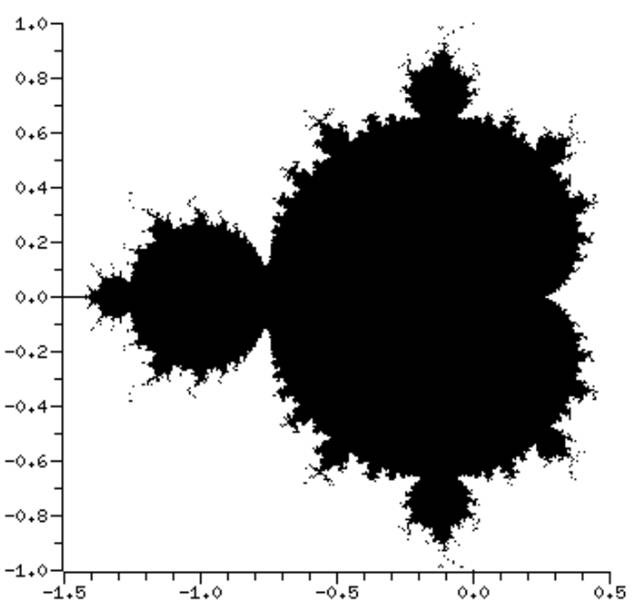
\includegraphics[width=0.5\textwidth]{fractal_2}
    \label{fig:Pou de Mandelbrot}
\end{figure} 
\end{minipage}%
\begin{minipage}{0.5\textwidth}
    \begin{figure}[h]
        \centering
        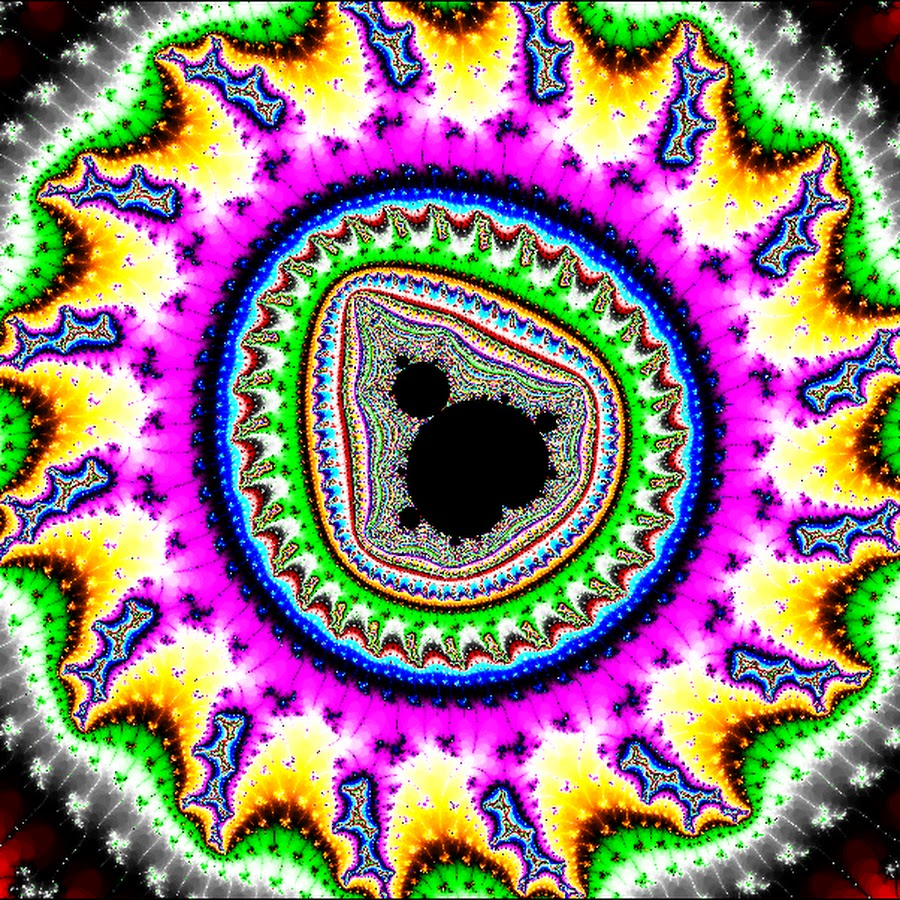
\includegraphics[width=0.5\textwidth]{mandel}
        \label{fig:pou de Mandelbrot colorié}
    \end{figure}
\end{minipage}
\end{frame}

\subsection{L'ensemble de Julia}
\begin{frame}
    \frametitle{L'ensemble de Julia}
    En Fixant maintenant une valeur de $c$ et en étudiant le comportement dynamique de chaque valeur de départ possible $z_0\in \mathbb{C}$. L'ensemble des valeurs de départ dont l'orbite est bornée sous itération de $Q_{c}$ forme l'ensemble rempli de Julia de $Q_{c}$ que l'on note $K(Q_{c})$. 
\begin{block}{Définition}
    Soit $c\in \mathbb{C}$. L'ensemble rempli de Julia de $Q_{c}$ est $K(Q_{c})=\left\{ z:|Q^{n}_{c}(z)| \nrightarrow \infty, \ n\to \infty \right\}$. 

     L'ensemble de Julia de $Q_{c}$ noté $J(Q_{c})$, est la frontière de cet ensemble. Le complément de l'ensemble de Julia est l'ensemble de Fatou $F(Q_{c})$.
\end{block}
\textbf{\underline{Remarque}}: A l'exception des cas où $c=-2$ et  $c=0$, l'ensemble de Julia de  $Q_c$ pour un  $c$ donné est un fractal.

\begin{minipage}{0.5\textwidth}
    \begin{figure}[h]
    \centering
    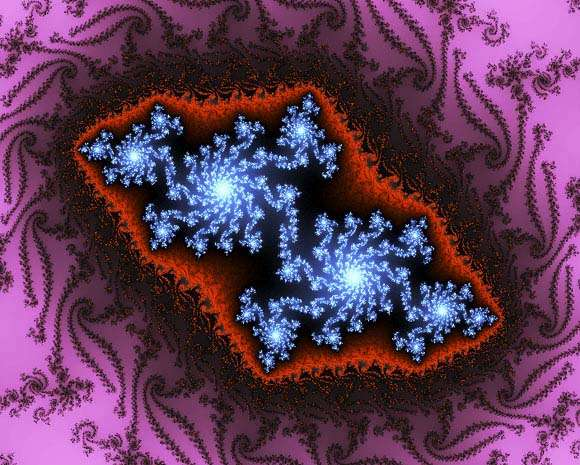
\includegraphics[width=0.5\textwidth]{mand126}
    \label{fig:fractal_5}
\end{figure}
\end{minipage}%
\begin{minipage}{0.5\textwidth}
\begin{figure}[h]
    \centering
    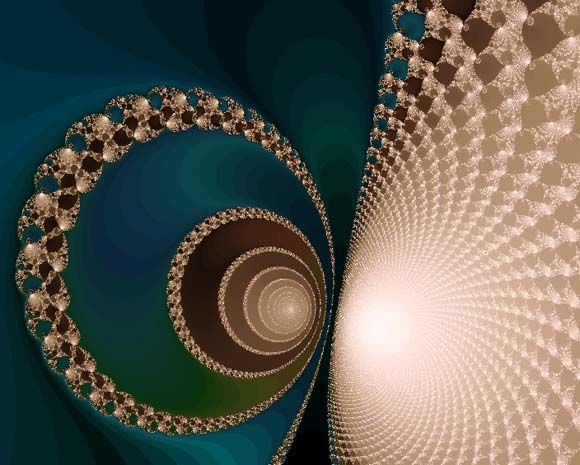
\includegraphics[width=0.5\textwidth]{mand41}
    \label{fig:mand41}
\end{figure}
\end{minipage}
\end{frame}

\section{Citations}

\begin{frame}
\frametitle{Citations}
\begin{itemize}
    \item \guillemotleft \ L'ensemble de Mandelbrot n'est pas une invention. C'est une découverte. Un peu comme le mont Everest est juste là. \guillemotright \ Roger Penrose
    \item \guillemotleft \ Demain, quelqu'un qui n'est pas familiarisé avec les fractales ne pourra pas être considéré comme scientifiquement instruit. \guillemotright John Archibald Wheeler (1911-2008) - Physicien expert en cosmologie et en physique quantique; proche de Niels Bohr et Albert Einstein.
    \item \guillemotleft  \ Les fractales sont importantes car elles ont permis de révéler un tout nouveau domaine des mathématiques, pertinent directement pour l'étude de la nature. \guillemotright \  Ian Stewart, professeur de mathématiques de l'université de Warwick en Angleterre.
    \item \guillemotleft  \ Lorsque les dessins de ces ensembles de Julia et Fatou sont apparus pour la première fois sur mon écran d'ordinateur, j'ai été frappé, non seulement par leur insondable complexité, mais aussi par leur extraordinaire beauté. Ils me semblaient à la fois totalement étranges et familiers comme si je les avais toujours connus. \guillemotright \ Benoît Mandelbrot
\end{itemize} 
\end{frame}

\section{Références}

\begin{frame}
\frametitle{Références}
\begin{itemize}
        \item Sources :

\url{http://villemin.gerard.free.fr/Wwwgvmm/Suite/Fractal.htm}

\url{http://charles.vassallo.pagesperso-orange.fr/fr/art/sommaire.html}

\vspace{0.5cm}

\href{https://www-fourier.ujf-grenoble.fr/~demailly/manuscripts/fractales-print.pdf}{Présentation de Jean-Pierre Demailly}
         le 19 novembre 2012, lors de la conférence au Lycée Champollion, Grenoble
\vspace{0.5cm}

\href{https://www2.mat.ulaval.ca/fileadmin/Cours/MAT-2430/Notes_de_cours/NotesDeCours.pdf}{Cours de Jean-Jacques Gervais}
         : \guillemotleft \ Introduction aux fractals et aux systèmes dynamiques \ \guillemotright \ Août 2009.

\vspace{0.5cm}

        \item Images :

Wikipédia: \href{https://fr.wikipedia.org/wiki/Ensemble_de_Mandelbrot}{Ensemble de Mandelbrot} et \href{https://fr.wikipedia.org/wiki/Ensemble_de_Julia}{Ensemble de Julia}
\url{http://charles.vassallo.pagesperso-orange.fr/fr/art/art_2.html}
\url{https://duckduckgo.com/?q=fractal&iax=images&ia=images}
        \item Vidéo:

\href{https://www.youtube.com/watch?v=Y4ICbYtBGzA}{Vulgarisation de l'ensemble de Mandelbrot réalisé par El Jj.}

\end{itemize}    

\end{frame}

\end{document}
